\documentclass{book}
\usepackage{amsmath}
\usepackage[most]{tcolorbox}
\usepackage{cleveref}
\usepackage{titlesec}
\usepackage{graphicx}
\usepackage{multirow}
\usepackage{array}

\graphicspath{ {./imagenes/} }

\titleformat{\chapter}[display]
  {\normalfont\bfseries}{}{0pt}{\Huge}

\tcbset{theostyle/.style={
    enhanced,
    sharp corners,
    attach boxed title to top left={
      xshift=-1mm,
      yshift=-4mm,
      yshifttext=-1mm
    },
    top=1.5ex,
    colback=white,
    colframe=black!75!black,
    fonttitle=\bfseries,
    boxed title style={
      sharp corners,
    size=small,
    colback=black!75!black,
    colframe=black!75!black,
  } 
}}

\newtcbtheorem{Definition}{Definición}{%
  theostyle
}{def}


\begin{document}

\begin{Definition}{}{ReadingTheManual}
  \textbf{Enlace covalente:} Enalce dado entre elementos no metálicos para formar \textbf{moléculas covalentes}. Los enlaces se forman ya que las moléculas \textbf{comparten} 
  electrónes para llegar a ser estables (\textit{cumplir la regla del octeto}).
\end{Definition}

\subsection{Enlaces sencillos, dobles, y tríples}

Vienen dados por el \textbf{número de electónes compartido}:

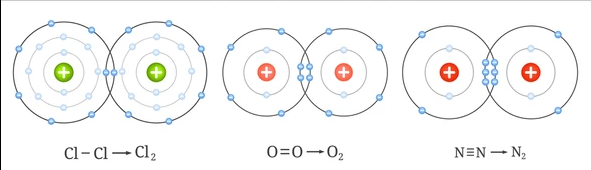
\includegraphics[scale=0.65]{enlaces-por-complejidad.png}

\section{Propiedades los enlaces covalenes}

\begin{tabular}{| c || m{2cm} | c m{8cm} |}
  \hline
  & Estado de agregación & Ejemplos & Propiedades generales \\
  \hline
  \multirow{2}{3em}{Elem.} & Molecular & 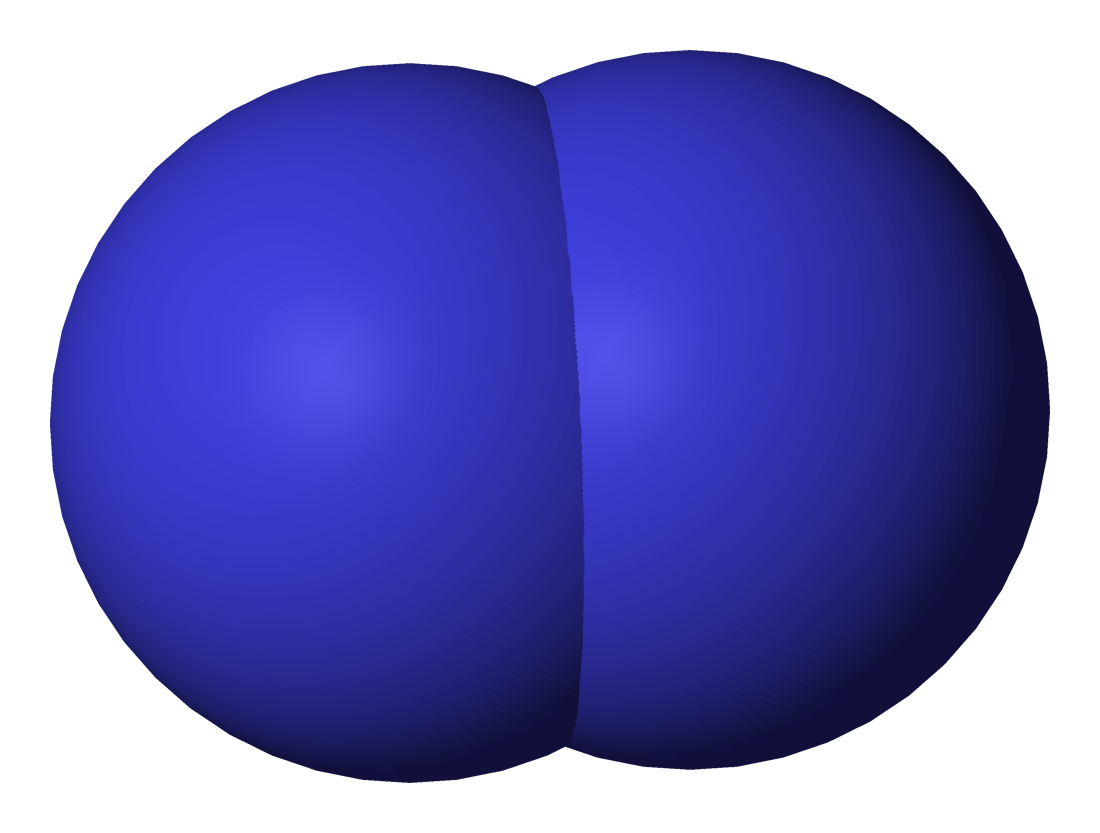
\includegraphics[scale=0.025]{dinitrogeno.png} \textit{$ N_{2} $} & Puntos de fusión y ebullición bajos (\textit{generalmente gases}),
                                                                                                              aislantes eléctricos (\textit{enlace fuerte, no hay electrones sueltos}), 
                                                                                                              insolubles en agua. \\ [1ex]
                           & Cristalino  & 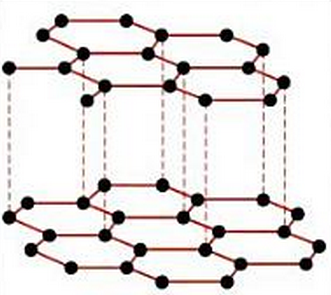
\includegraphics[scale=0.1]{grafito.png} \textit{$ C $} & Sólidos*. \\ [1 ex]
  \hline
  \multirow{2}{3em}{Comp.} & Molecular & \includegraphics[scale=0.025]{cloruro de hidrógeno.png} \textit{$ HCl $} & Puntos de fusión y ebullición bajos (\textit{gases, líquidos, y sólidos}),
                                                                                                                     malos conductores eléctricos, insolubles en agua pero sí en medios orgánicos.\\

                           & Cristalino  & 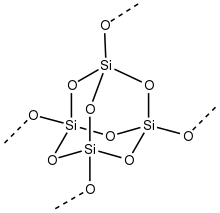
\includegraphics[scale=0.15]{dioxido de silicio.png} \textit{$ SiO_{2} $} & Duros, aislantes eléctricos, insolubles en agua.  \\ [2 ex]
  \hline
\end{tabular}
* Demas características dependen del elemento (carbono, silicio...), y de su estructura (laminal, tetrahédrica...):

\begin{itemize}
  \item \textbf{Diamante:} Estructura tetrahédrica de carbonos. No conduce la electricidad. $ \iff $ Es la conexión más dura que se conoce (\textit{no hay electrones sueltos}).
  \item \textbf{Grafito:} Redes laminales de carbonos. Conduce la electricidad. $ \iff $ Es blando (\textit{los electrones son libres entre láminas}).
\end{itemize}

\end{document}